\newpage
\section{Durchführung}
\label{sec:Durchführung}
Mit Hilfe der in Abbildung \ref{fig:Versuchsaufbau} dargestellten Versuchsapperatur sollen zwei
Spektrallinien des Elements Cadium untersucht werden. Dazu wird eine Cd-Lampe mit einem Magnetfeld
durchsetzt und ihre Aufspaltung untersucht. Wie aus der Abbildung
bekannt, wird nur der transvertale Anteil des Lichts mit Hilfe von Linsen kollimiert.
Das Geradsichtprisma spaltet das Licht in seine spektralen Bestandteile auf.
Mit dem darauf folgenden Spalt und Polarisationsfilters kann die zu untersuchende Spektrallinie ausgewählt werden.
Diese Spektrallinie wird dann auf die Lummer-Gehrcke-Platte fokussiert und erzeugt dort ein Interferenzmuster,
welches mit der Digitalkamera regestriert wird.
Wichtige Kenngrößen sind hier das Dispersionsgebiet
\begin{equation}
    \label{eqn:disp}
    \Delta \lambda_\text{D} = \frac{\lambda^2}{2 \cdot d \sqrt{n^2-1}}
\end{equation}
und das Auflösungsvermögen
\begin{equation}
    \label{eqn:auf}
    A = \frac{\lambda}{\Delta \lambda} = \frac{L \cdot \left(n^2 - 1\right)}{\lambda},
\end{equation}
mit der Wellenlänge $\lambda$, des Brechungsindexes $n$, der Länge der Platte $L$ und der
Dicke der Platte $d$.
\begin{figure}[htb]
  \centering
  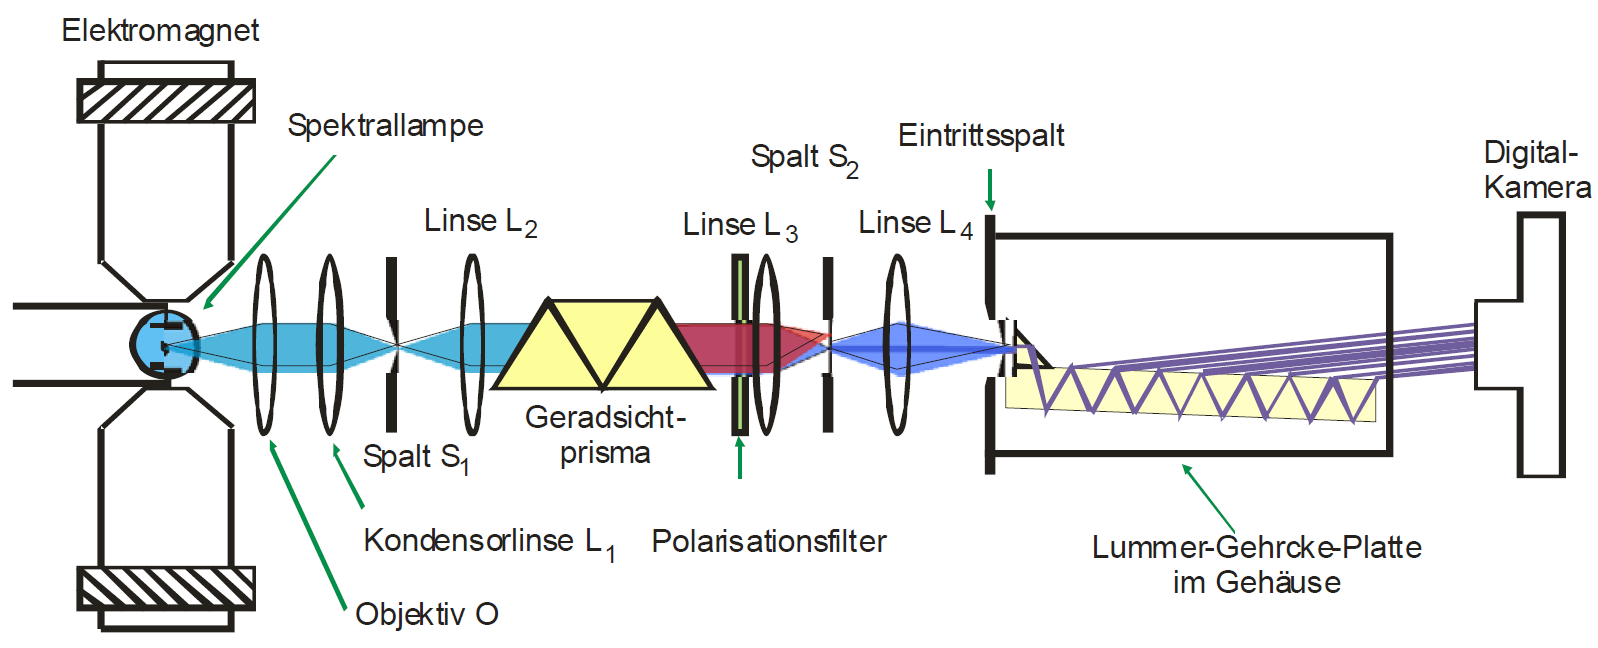
\includegraphics[width=\textwidth]{content/pictures/Versuchsaufbau.png}
  \caption{Schematische Darstellung des verwendeten Versuchsaufbaus. \cite{anleitung_alt}}
  \label{fig:Versuchsaufbau}
\end{figure}

Eine genaue Messung der Aufspaltung erfordert gute Kenntnisse über das verwendete $B$-Feld.
Aus diesem Grund wird zunächst eine Kalibration des verwendeten Feldes durchgeführt, hierzu wird das
Magnetfeld in Abhängigkeit von fließendem Strom gemessen. 
Das aus der Cd-Lampe austretende Licht wird mit dem Objektiv und der Linse $\text{L}_1$ möglichst
scharf auf den Spalt $\text{S}_1$ abgebildet.
Nun wird mit Hilfe der Linse $\text{L}_2$ das Lichtbündel so eingestellt, dass es parallel und mit dem maximalen
Durchmesser des Geradenprismas auf jenes fällt. Das aus dem Geradenprisma austretende Licht wird mit der 
Linse $\text{L}_3$ auf den zweiten Spalt $\text{S}_2$ abgebildet, mit diesem Spalt kann dann eine der Spektrallinien
ausgewählt werden. Mit der Linse $\text{L}_4$ wird die ausgewählte Linie auf den Eingang der Lummer-Gehrcke-Platte
fokussiert und zwar so, dass der gesamte Eintrittsspalt ausgefüllt ist. 
Mit dem Polarisationsfilter kann dann weiter noch die Polarisation ausgewählt werden. Nun wird 
mit der Digitalkamera das Interferenzmuster aufgenommen. Einmal ohne Aufspaltung und einmal 
mit Aufspaltung, also eingeschaltetem $B$-Feld. Dabei soll der Wert des $B$-Feldes jeweils so
gewählt werden, dass die $\symup{\pi}$ also auch die $\symup{\sigma}$-Übergänge beobachtet werden können.
Diese Prozedur soll einmal für die blaue und einmal für die rote Spektrallinie des Cadiums geschehen.
Dazu muss für jede Linie die Ausrichtung der optischen Elemente ab $\text{L}_3$ neu eingestellt werden.
\FloatBarrier